\subsection{WCM Definitions}


\subsubsection{Dynamic Lists}

You will hear the term `dynamic list' quite frequently when working
with a site studio site.  A dynamic list is the listing generated by
doing a query against the content server.  For example I might do a
query for all the latest report documents, like so:

\begin{verbatim}
dDocType <matches> `report'
\end{verbatim}

\subsubsection{Page Templates}

Fully-formed HTML files that define the layout and high-level
look-and-feel of web pages, including the placement of contribution
regions (that is, editable areas on the page), navigation aids (in the
form of fragments) and site-wide images (banners and the like). Page
templates are the highest-level site design object.

Page Templates are at the top of the hierarchy. They provide the
framework for the pages in a Web site within which the site content is
displayed. In addition to standard HTML layout and formatting code,
they contain site-wide images and other assets, and tags for fragments
and/or placeholders. Page templates are stored and managed on the
content server.

\subsubsection{Subtemplates}

Subtemplates are the same as page templates, but with one important
difference: subtemplates do not have <HTML>, <HEAD>, and <BODY>
tags. As such, they are essentially chunks of HTML code that can be
inserted in page templates.

Partial HTML files (that is, without head and body sections) that can
be inserted into placeholders on page templates to divide them into
further smaller, reusable areas with their own placeholders and
contribution regions.

A subtemplate is a partial HTML file (that is, without a head and body
section) that provides a mechanism to divide a placeholder on a page
template into further smaller, reusable areas with their own
placeholder(s). There is a circular relationship between placeholders
and subtemplate; that is, a placeholder may contain a subtemplate,
which, in turn, may include one or more placeholders. Subtemplates are
stored and managed on the content server.

\subsubsection{Element Definitions}

Files that define the editing experience for element
types. Specifically, they specify what a contributor can do when
editing an element.

Elements are the smallest chunks of reusable information in a Site
Studio Web site. They are referenced in region templates, which causes
their data to be pulled into the region template using the layout and
presentation defined in the template. A region template may contain
multiple element references. There are no files associated with
elements as such; that is, there are no "element files" on the content
server. Groups of elements are arranged in region definitions, which
specify site content types. Elements are controlled by element
definitions, which specify the editing experience available to
contributors for an element type. Specifically, they set the available
editing features in the Contributor editor when a contributor is
editing elements in a contributor data file.


\subsubsection{Region Definitions}

Think of it as a Type of Content for example a Press Release.  A press release may consist of a title, an image, and a body.  So a region definition will specify three elements that are of types: ‘text-only’ = title, ‘image’, and ‘wysiwig’=body.

Files that define the type of content that elements of a particular type consists of. They also specify the content creation and switching options available to contributors for contribution regions, and set default metadata for content files associated with these regions.

\begin{figure}[h!]
  \centering
  \fbox{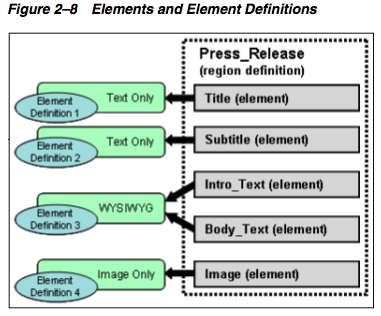
\includegraphics[width=130mm]{images/ElementsAndElementDefinitions}}
  \caption{Elements and Element Definitions}
\end{figure}



\subsubsection{Region templates}

Region Templates are associated with Region Definitions.  They don’t
need to use all the elements specified in a Region Definition.  For
example you could have a teaser page and then a link to the full page.
2 Region Templates, 1 Region Definition and 1Data File.

Partial HTML files (that is, without head and body sections) that
define the layout and look-and-feel of the data in contribution
regions within web pages.

A region template is a partial HTML file (that is, without a head and
body section) that defines the layout and look-and-feel of the data in
a contribution region (marked on a page template using a placeholder
tag). Region templates are controlled by region definitions, which
define what kind of content can go in the region template. They also
specify the content creation and switching options available to
contributors for the contribution region, and set default metadata for
content files associated with the region. Both region templates and
region definitions are stored and managed as separate assets on the
content server. A region template may have one or more references to
elements.

\begin{figure}[h!]
  \centering
  \fbox{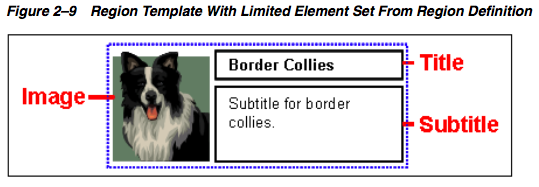
\includegraphics[width=130mm]{images/regTempWithLimitedElementSet}}
  \caption{Region Template with limited element set from region definition}
\end{figure}

\begin{figure}[h!]
  \centering
  \fbox{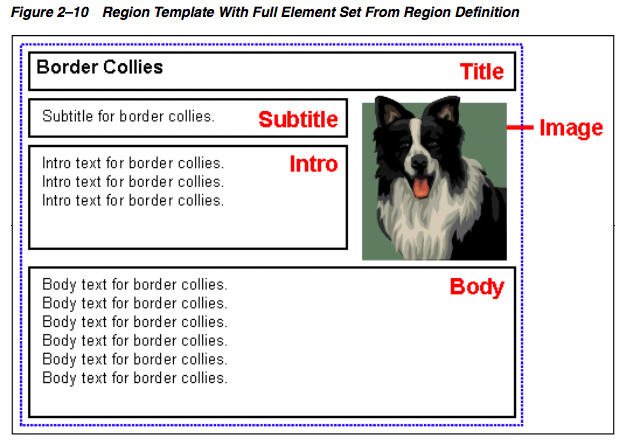
\includegraphics[width=130mm]{images/regTempWithFullElementSet}}
  \caption{Region Template with limited element set from region definition}
\end{figure}


\begin{figure}[h!]
  \centering
  \fbox{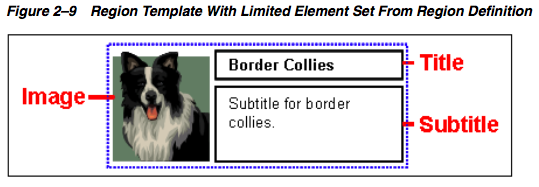
\includegraphics[width=130mm]{images/regTempWithLimitedElementSet}}
  \caption{Region Template with limited element set from region definition}
\end{figure}

\subsubsection{Contributor data files}

Content files in XML format that are generated by Site
Studio. Contributor data files are edited using the Site Studio
Contributor application.

\subsubsection{Native documents}

Content files created using familiar third-party applications such as
Microsoft Word. Native documents are converted to HTML format using
Dynamic Converter, and they are edited using their associated
application.

\subsubsection{Placeholder Definitions}

Files that define what region definitions, region templates, and
subtemplates are allowed for the associated placeholders. They also
specify what contributor actions are allowed for the placeholders.

A placeholder is no more than an insertion point (a tag) on a page
template to identify where there is a contribution region (that is,
editable area) on the web page. What that contribution region contains
and what it looks like is defined using region templates and region
definitions. A page template may contain multiple placeholders. There
are no files associated with placeholders; that is, there are no
"placeholder files" on the content server. Placeholders are controlled
by placeholder definitions, which specify what content can go in the
contribution region and how it is displayed, as well the actions
available to contributors (for example, switching content or modifying
metadata). A placeholder contains either one subtemplate or one region
template.


\subsubsection{Fragment libraries}

Collections or chunks of code (fragments) that enhance the
functionality of a Site Studio Web site (for example, by providing
dynamic navigation aids or a standard page footer).

They are chunks of code that can be added to a page template to enhance its
functionality. Site Studio comes with several predefined fragments
(for example, for dynamic navigation aids), but you can also create
your own fragments. A page template may contain multiple
fragments. Fragments are stored in fragment libraries.

\subsubsection{Manager configuration settings}

Files that define the functionality that is available in Site Studio
Manager. Manager is a web-based tool that allows designated users
(site managers) to modify the structure of a Web site.

\subsubsection{Conversion Definitions}

Files that specify the conversion rules for native documents on a Web
site.